%% Template for MLP Coursework 4

%% Based on  LaTeX template for ICML 2017 - example_paper.tex at 
%%  https://2017.icml.cc/Conferences/2017/StyleAuthorInstructions

\documentclass{article}
\usepackage[T1]{fontenc}
\usepackage{amssymb,amsmath}
\usepackage{txfonts}
\usepackage{microtype}
\usepackage{xspace}
\xspaceaddexceptions{\%}

% Lists with less spacoing between items
\usepackage{paralist}

% For figures
\usepackage{graphicx}
\usepackage{subfig} 

% For citations
\usepackage{natbib}

% For algorithms
\usepackage{algorithm}
\usepackage{algorithmic}

% the hyperref package is used to produce hyperlinks in the
% resulting PDF.  If this breaks your system, please commend out the
% following usepackage line and replace \usepackage{mlp2017} with
% \usepackage[nohyperref]{mlp2017} below.
\usepackage[hyphens]{url}
\urlstyle{same}
\usepackage{hyperref}

% Packages hyperref and algorithmic misbehave sometimes.  We can fix
% this with the following command.
\newcommand{\theHalgorithm}{\arabic{algorithm}}


% Set up MLP coursework style (based on ICML style)
\usepackage{mlp2019}
\mlptitlerunning{MLP Coursework 3 -- Interim Report (\groupNumber)}
\bibliographystyle{icml2017}


\DeclareMathOperator{\softmax}{softmax}
\DeclareMathOperator{\sigmoid}{sigmoid}
\DeclareMathOperator{\sgn}{sgn}
\DeclareMathOperator{\relu}{relu}
\DeclareMathOperator{\lrelu}{lrelu}
\DeclareMathOperator{\elu}{elu}
\DeclareMathOperator{\selu}{selu}
\DeclareMathOperator{\maxout}{maxout}






%% You probably do not need to change anything above this comment
\usepackage{minted}
\newminted{python}{frame=lines,framerule=2pt}

%% REPLACE this with your project title, group ID and list of student numbers for the group
\def\projectTitle{Title}
\def\groupNumber{G014}
\def\studentNumbers{s2196789, s2163307}

\begin{document} 

\twocolumn[
\mlptitle{\projectTitle: Image and Vision Computing Mini-Project}

\centerline{\groupNumberz}

\vskip 7mm
]

%The abstract should be a few sentences (100--200 words) long,  providing a concise summary of the contents of your report including the key research question(s) addressed, the methods explored, the data used, and the findings of the experiments.
\begin{abstract} 
In this report, we investigate the effect of perturbations on a classical and a deep learning method as applied to image classification.  Two classifiers are trained with the FER-2013 dataset, one based on a support-vector machine (SVM), and the other based on a pretrained ResNet18 architecture. We achieve 48.97\% test accuracy using a SVM and 57.40\% using the ResNet18. To test the robustness of these two models, we then generate a new test dataset by applying 8 typical image transformations with increasing perturbation respectively from the original test images. In the experiment, it can be observed that though both models are invariant to pixel noises and brightness adjustment, image blurring, occlusion and contrast adjustment may have a negative effect on their accuracy performance.

\end{abstract} 

%This document provides a template for the MLP coursework 4 final report.  This template structures the report into sections, which you may use, or you can structure it differently if you wish.  If you want to use subsections within a section that is fine. In this template the text in each section will include a very brief outline of what you should include in each section, along with some practical LaTeX examples (for example figures, tables, algorithms).  Your document should be no longer than \textbf{eight pages},  with an additional page (or more!) allowed for references.

%You should give a broad introduction to the project, including citations to related work. Your aim here is to explain why the project is addressing an interesting topic, and how it relates to things that have been done in the area.

%You should make clear what are the aims and objectives of the project, what are the research questions being addressed. Are they verifiable by experiments and worth conducting research on? Be precise. In this section you should make clear what the project's contribution is: how is it different to what is already done.  If the project objectives have changed since the interim report, please point this out and discuss why it was so.

%Use bibtex to organise your references -- in this case the references are in the file \verb+example-refs.bib+.  Here is a an example reference \citep{langley00}. 


\section{Introduction}
\label{sec:intro}
In this report we focus on the performance of two image classification methods. A classical method, Support Vector Machine (SVM) and a deep learning method, Resnet-18 are examined by evaluating their accuracy on baseline test set and on test images with some perturbations added to. We first start with reviewing some published articles about both SVM using HOG features and Resnet-18. We find that HOG features are efficiently helping classifiers determine the right categories for images. We also evaluate the characteristics of Resnet and how it distinguishes itself by achieving 90\%+ accuracy on CIFAR10\footnote{https://www.kaggle.com/kmldas/cifar10-resnet-90-accuracy-less-than-5-min}. 
Then we use HOG features extracted from training images to train SVM and use raw images to fine-tune Resnet-18. After getting good validation accuracy for both classifiers, we add some perturbations to the test set and compare it with the accuracy without perturbations. We conclude that both classifiers are robust to small perturbations while they cannot overcome the challenges where the perturbations are significant.

\section{Data set and task} 
\subsection{FER-2013 dataset}
The dataset we used consists of 35,887 images of 7 emotions, which are angry, disgust, fear, happy, surprise, neutral, and sad. Each image has grayscale $48\times48$ pixels and has been automatically registered so that each face occupies the same amount of space \cite{jumani2019facial}. The data set was divided into two subsets, training set and public test set. The training consists of 28,709 examples and the test set consists of 7,178 examples.

\subsection{Training SVM and ResNet18}
Our first task aims to learn facial expressions from those images. To complete this task, we will train SVM and ResNet-18 respectively based on the given dataset. The classifiers are expected to be able to successfully identify the emotion from seven categories given an image with high accuracy.

\subsection{Robustness Exploration}
After the SVM and ResNet image classifiers are well-trained, our second task is to examine the robustness of individual models. The performance of a model tested on the FER-2013 test dataset is used as the base case. A new dataset used for robustness test is derived from the test dataset by applying a variety of perturbations. The techniques include 8 typical image transformations which are adding \textbf{Gaussian pixel noise}, applying \textbf{Gaussian blurring}, increasing/decreasing \textbf{image contrast}, increasing/decreasing \textbf{image brightness}, adding \textbf{occlusion} and adding \textbf{salt and Pepper noise}. For each disruption scenario, 10 increasing levels of perturbation are applied to the original images. The robustness of these two classifiers will be evaluated by re-calculating their classification accuracy based on the perturbed dataset. 

% Explain clearly the technical methodology, the models and algorithms that are used.  Approaches that were covered in the lectures can be described briefly, but if you are using modifications to such approaches make sure these are clearly described and self-contained. Again use citations to the literature.
% If you present algorithms, you can use the \verb+algorithm+ and \verb+algorithmic+ environments to format pseudocode (for instance, Algorithm~\ref{alg:example}). These require the corresponding style files, \verb+algorithm.sty+ and \verb+algorithmic.sty+ which are supplied with this package. 

\section{Methodology}


\subsection{Extracting Image Features for SVM}
In this section, we will explain how the feature descriptor for face images using \textbf{Histogram of Gradients} and \textbf{face landmarks} can be developed and used for SVM training and testing.

\subsubsection{Histogram of Oriented Gradients (HOG)}
Histogram of oriented gradient (HOG features) is used to calculate the histogram of gradient direction of local area of the image. According to \cite{Dalal2005HistogramsOO}, HOG features can extract facial emotional features effectively. In this experiment, the implementation process of obtaining the HOG description operator will be explained in the following steps (with visualisations): 
\begin{itemize}
\item Calculating image gradient:  

To filter the colour or intensity data of the image, two filter kernels are used to convoluted with the image to calculate the vertical and horizontal gradients of an image. The Sobel filter used to extract vertical edges is $[-1,0,1]^T$ and the one for horizontal edges is $[-1,0,1]$. 

\item Calculating magnitude and orientation of the image gradients: 

Assume that $dx$ and $dy$ represent the gradient values in X-direction and Y-direction of an image which was obtained in the previous step. We can compute the magnitude and orientation of the image using the following equation.
\begin{align*}
Magnitude(\mu) & = \sqrt{(dx)^2+(dy)^2}\\
Angle(\theta) & =  tan^{-1}(\frac{dy}{dx})
\end{align*}

\item Computing gradient histograms for each block:

After obtaining the gradient matrices (magnitude and angle matrix) for each pixel, one image ($48\times48$ pixels) will be divided into 9 cells which have the size of $16\times16$ pixels. And in this experiment, each cell itself is a block. For each cell, the magnitude values of these 256 pixels are binned and cumulatively added into 8 buckets of unsigned direction which is from 0 - 180 degree.

For example, to update a 8-bin histogram, the given magnitude and the angle of one pixel are $\theta$ and $\mu$.  The corresponding bin numbers which are to be modified are $j$ and $j+1$. The value of j is:
\begin{align*}
j & = floor(\frac{\theta}{\Delta \theta}-0.5)\\
\text{where} \; \Delta \theta &= \frac{180}{\text{number of bins}}
\end{align*}

The magnitude $\mu$ will be divided into 2 portions ($V_j$ and $V_{j+1}$) and assigned to the $j^{th}$ and $(j+1)^{th}$ bins. $C_j$ and $C_{j+1}$ are the degree values of the each bin's centre.
\begin{align*}
V_j & = \mu(\frac{C_{j+1} - \theta}{\Delta \theta})\\
V_{j+1} &= \mu(\frac{\theta - C_{j}}{\Delta \theta})
\end{align*}

Therefore, for each block in the image, a 8-point feature vector is collected.
\item Block normalisation:

Since the block has the same size with the cell ($16\times16$ pixels), the 8-point feature vector can be represented as:
\begin{align*}
f b_i & = [b_1,b_2, ..., b_{16}]
\end{align*}
After applying the $L_2$ norm to $f b_i$, we can get the normalised vector ($\epsilon$ is a small value to avoid division by zero error):
\begin{align*}
f b_i & = \frac{f b_i}{\sqrt{||f b_i||+\epsilon}}
\end{align*}
In our case, because each image has 9 blocks and each block is represented as a 8-point feature vector, the final HOG feature vector (one-dimensional) of the whole image has a length of 72.

\end{itemize}
The figures below visualise the intermediate stages of extracting HOG features.
\begin{figure}[H]
    \centering
    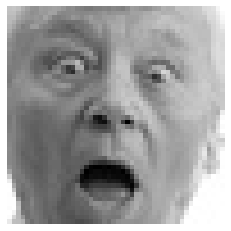
\includegraphics[height=1in]{HOG figures/original.png}
    \caption{Original image}
\end{figure}

\begin{figure}[H] 
    \centering
    \subfloat[Horizontal Gradients]{%
        \quad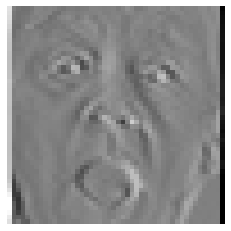
\includegraphics[height=1in]{HOG figures/dx.png}\quad%
        }%
    \hspace*{.4in}
    \subfloat[Vertical Gradients]{%
    \quad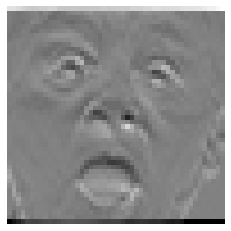
\includegraphics[height=1in]{HOG figures/dy.png}\quad%
        }%
    \caption{Image Gradients}
\end{figure}

\begin{figure}[H] 
    \centering
    \subfloat[Magnitude]{%
        \quad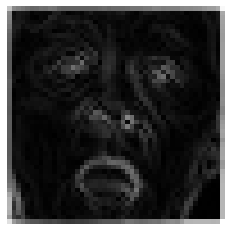
\includegraphics[height=1in]{HOG figures/mag.png}\quad%
        }%
    \hspace*{.4in}
    \subfloat[Orientation]{%
    \quad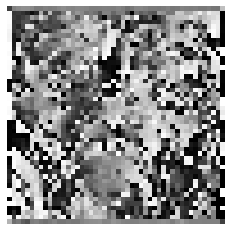
\includegraphics[height=1in]{HOG figures/ang.png}\quad%
        }%
    \caption{Magnitude and Orientation}
\end{figure}

\begin{figure}[H]
    \centering
    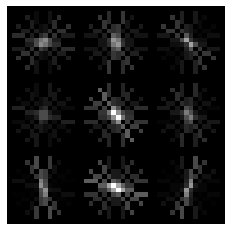
\includegraphics[height=1in]{HOG figures/hog.png}
    \caption{HOG Features}
\end{figure}

\subsubsection{Facial Landmarks}
To extract facial landmarks, the first step should be localising the face(s) in the image. In FER-2013 dataset, since all the faces are adjusted to be in the center of images and they occupy almost same amount of space \cite{jumani2019facial}, this step can be omitted. Therefore, we can extract the landmarks  directly by applying \textbf{Dlib}'s facial landmark detector on the images. The pretrained detector will map facial structures on the face which consists of 68 (x, y)-coordinates \cite{8696059}. Figure \ref{dlib} below shows the a face with landmarks on it.

\begin{figure}[H]
    \centering
    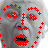
\includegraphics[height=1in]{figures/dlib.png}
    \caption{Face with landmarks}
    \label{dlib}
\end{figure}

After the locations of 68 key landmarks are obtained, these features will be flattened as a one-dimensional vector, which can be represented as:
\begin{align*}
f l_i & = [x_1,y_1,x_2,y_2, ..., x_{68},y_{68}]
\end{align*}

To combine the facial landmarks and the HOG features, we can simply concatenate these 2 one-dimensional vectors. Finally, each image can be represented as a vector which has the length of 208 and then fed into SVM model for both training and testing.


\subsection{Resnet-18}

The other classifier we used is Resnet-18. We need to fine-tune Resnet-18 to fit the model of our problem. As its name informed, Resnet-18 is an 18-layer residual neural network which achieves high accuracy on image recognition tasks. 

\subsubsection{Architecture of Resnet}

Resnet-18 consists of one convolutional layer \textbf{conv1} which takes input units downsampling with stride 2, and four basic blocks with each block having two hidden convolutional layers. After convolutional layers, it adds an \textbf{average pool} layer followed by a \textbf{fully connected} layer and a \textbf{softmax} layer. Figure \ref{fig:Resnet18_architecture} shows the details of Resnet-18 architecture. 

\begin{figure}[htp]
    \centering
    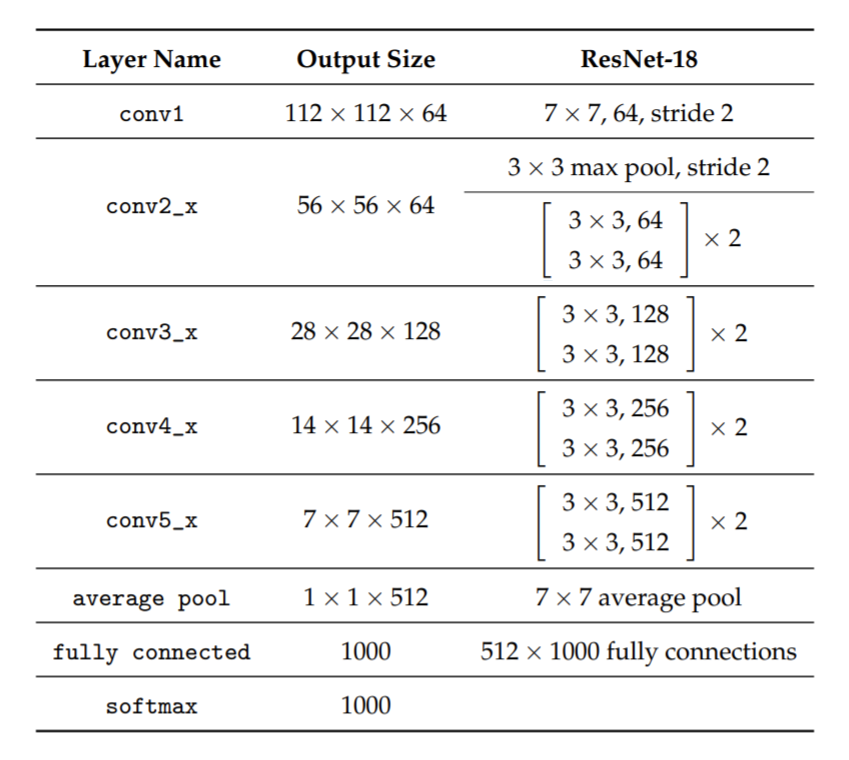
\includegraphics[width=\columnwidth]{figures/Resnet18_architecture.png}
    \caption{Resnet18 architecture}
    \label{fig:Resnet18_architecture}\citep{Resnetarch}
\end{figure}

\subsubsection{Fine-tune Resnet-18}

In our task we need to identify images from 7 categories. There are some settings that need to be modified in the pretrained model. According to figure \ref{fig:Resnet18_architecture}, the \textbf{fully connected} layer has output size of 1000. We modified it to 7 using the following code. 

\begin{verbatim}
fc_features = model.fc.in_features
model.fc = nn.Linear(fc_features, 
            len(IMAGE_CATEGORIES))
\end{verbatim}

The pretrained model takes colored pictures as input, which have 3 channels. Our dataset are all grayscale which only have one channel. The following code changes the \textbf{conv1} layer to make it accept one chaannel image.

\begin{verbatim}
model.conv1= nn.Conv2d(1, 64, kernel_size=(7,7), 
stride=(2,2), padding=(3,3),bias=False)
\end{verbatim}

Since it took very long time to retrain the whole model, a better approach is to freezing the convolutional layers and only retrain the fully connected layer. The pseudocode for achieving this are showed in the following algorithm.

\begin{algorithm}[ht]
\begin{algorithmic}
   \FOR{$param$ {\bfseries in} $conv\ layer$}
   \STATE set param grad to false
   \ENDFOR
   \FOR{$param$ {\bfseries in} $fc\ layer$}
   \STATE set param grad to true
   \ENDFOR
\end{algorithmic}
\end{algorithm}

For the gradient of parameters in convolutional layer, we set it to \textit{false} because we don't want backward propagation to update the weights. On the other hand, we do want the backward propagation on \textbf{fully connected} layer to update its weight, hence we set its gradient to \textit{true}.

\subsection{Generating the Perturbed Dataset}
To investigate how robust the two trained classifiers are, 8 set of perturbed image data are generated for testing. For the convenience of explaining how image are perturbed using different, we denote the original image as $I$ and perturbed image as $I^{'}$, where both $I$ and $I^{'}$ are $48 \times 48$ 8-bit greyscale images and the pixel intensity ranges from 0 to 255.

\begin{itemize}
    \item Add Gaussian pixel noise
    
    First, a mask $M$ with the same size of the original image is created, where each element in the mask is a Gaussian distributed random number. The mean of the Gaussian distribution is fixed to 0, while the standard deviation increases with the perturbation level. The image with Gaussian pixel noise can be represented as:
    \begin{align*}
    I^{'} & = I+M
    \end{align*}
    
    \item Gaussian blurring
    
    The idea of Gaussian blurring is filtering the image with a mask which approximate a Gaussian. The given filter kernel is a $3 \times 3$ matrix:
    \begin{align*}
    f & = \frac{1}{16}\begin{bmatrix}
            1 & 2 & 1\\
            2 & 4 & 4\\
            1 & 2 & 1
            \end{bmatrix}
    \end{align*}
    
    The output image after successive Gaussian blurring is:
    \begin{align*}
    I^{'} & = f^n * I \\
    \end{align*}
    where $n$ represents how many times we should convolve the image with the mask.
    
    \item Image Contrast Increase/ Decrease
    
    Suppose $\alpha$ is the contrast ratio. If $\alpha > 1$, it will lead to an increase in the image contrast, else it will decrease the image contrast. After adjusting contrast, the output image is: 
    \begin{align*}
    I^{'} & = \alpha I
    \end{align*}
    
    \item Image Brightness Increase/ Decrease
    
    Suppose $\beta$ is the amount of brightness that should be added/subtracted on the image. If $\beta > 0$, it will lead to an increase in the image brightness, else it will decrease the image brightness. After adjusting brightness, the output image is: 
    \begin{align*}
    I^{'} & = I + \beta
    \end{align*}
    
    \item Occlusion of the Image Increase
    
    Image occlusion is to select a part of the image and decrease the pixel intensities in this region to 0. In this experiment, occlusion region's shape is square and its edge length increases with the perturbation level. Suppose the coordinates of the left-upper corner is randomly selected as $(x, y)$ and its edge length is $l$. The output image after occlusion is:
    \begin{align*}
    I^{'} \leftarrow I[x:x+l,y:y+l] = 0
    \end{align*}
    
    Note that $(x+l)$ or $(y+l)$ may exceed the boundary of original image. So when generating random $x$ and $y$, they should be in the range of $[1, 48-l]$.
    
    \item Salt and Pepper Noise
    
    Salt and pepper noise is a kind of impulse noise. The original value of the pixel is replaced by extreme values $smin$ and $smax$ equal to the dynamic range of the image pixel value. For an 8-bit grayscale image in our experiment, $smin=0$ and $smax=255$ \cite{leavline2013salt}. The noise amount increases with the perturbation level.

\end{itemize}

Finally, we also make sure the pixel values are integers in the range [0,255] after the perturbed image $I^{'}$ is created.

\section{Experiments}
\label{sec:expts}

In the experiment we trained two classifiers firstly. In order to achieve higher accuracy and prevent our model from overfitting, we split the training set into training set and validation set at ratio of 0.75 and 0.25. The validation set are used to tune hyperparameters of the models. Then we added a variety of pertubations to pixels to test robustness of our models.

\subsection{Training models}

\subsubsection{SVM}
 The SVM classifier is trained using HOG features extracted from training set. We extracted hog features for both training set and validation set and we using hog features of validation set to adjust HOG features' hyperparameters and evaluate the performance of our model. The hyperparameters are including \textbf{orientations}, \textbf{pixels per cell}, and \textbf{cells per block}. In this experiment we will always use 8 as the number of orientations because it provides enough details of features in each cell. 
 
A SVM classifier is fitted with HOG features of training set and we evaluated its performance on validation set. We tried a number of combinations of pixels per cell and cells per block hyperparameter to decide the best combination. The results are showed in figure \ref{fig:SVM_HOG_Feature} compared with two dummy classifiers.

\begin{figure}[htp]
    \centering
    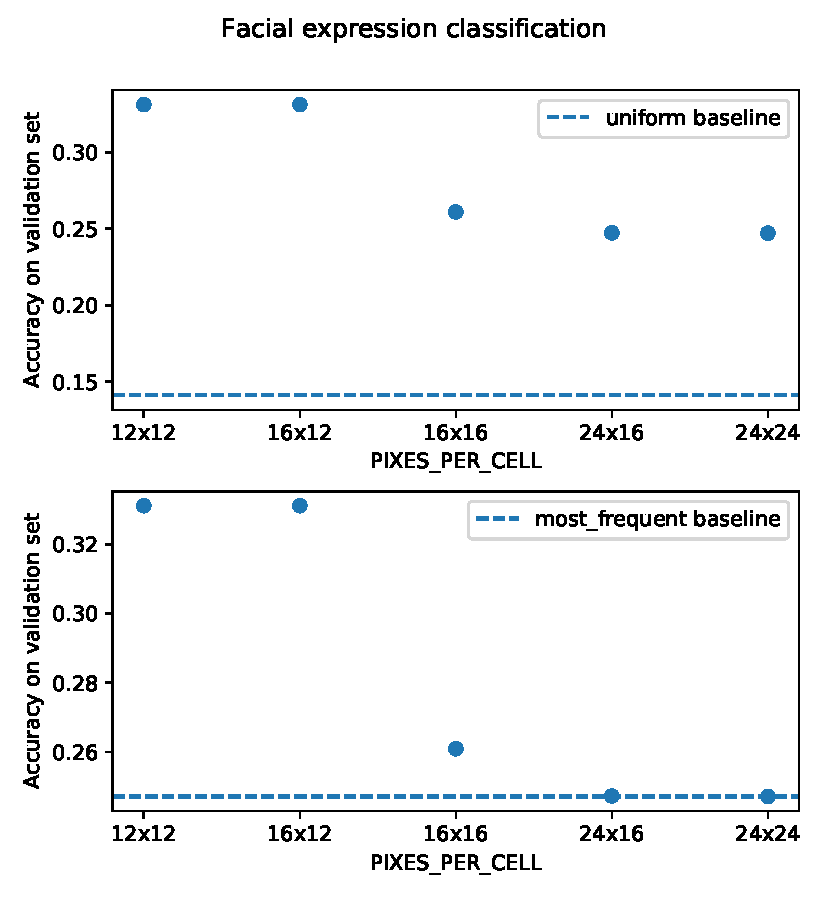
\includegraphics[width=\columnwidth]{figures/SVM}
    \caption{Different learning rate versus Accuracy on validation set for SVM classifier with HOG features}
    \label{fig:SVM_HOG_Feature}
\end{figure}

Those two dummy classifiers include a uniform baseline, which randomly guesses one category for each image, with accuracy of roughly $\frac{1}{7}$, and a most-frequent baseline, which takes label of image with the largest number as output, with accuracy of 0.247. According to figure \ref{fig:SVM_HOG_Feature}, we could find that the accuracy on validation set decreases as we increase the number of pixels per cell. When the number of pixels becomes more than $24\times16$, the accuracy is even lower than the most frequent baseline. 

When the number of pixels per cell is $12\times12$ or $16\times12$, the accuracy on validation set reaches more than 0.3. However the performance still not satisfying, and then we implemented HOG features with \textbf{Dlib}'s facial landmark detector. The trained facial landmarks are directly downloaded from dlib.net with which we used to generate training set landmarks and concatenate with HOG features. We also tested the performance using landmarks with different setting of hyperparameters and we got similar results for both $12\times12$ and $16\times16$. Considering the training time of $12\times12$ is far longer than that of $16\times16$, finally we chose $16\times16$ as the hyperparameter setting for our model. As a result we got accuracy of 0.49 on test set.

\subsubsection{ResNet-18}
In the training process of ResNet-18, we used a pretrained model from pytorch and then fine-tuned the model by freezing convolutional layer and re-train the fully connected layer. ResNet-18 is an 18-layer neural network with many parameters which takes very long time to train. Using pretrained model could help us save a lot of time while improving the accuracy by using the obtained weights and architecture and applying the learning on our problem. 

The pretrained model has 1000 outputs, which means it can identify 1000 categories. We changed it to 7 to fit our model. In addition, we changed the first convolutional layer of the pretrained model to make it accept one channel image as input. We set the loss function for our model to be cross entropy loss and used stochastic gradient descend to minimize the loss function. In the process of training model, a list of learning rates has been experimented by training 100 epoch for each of the learning rate and their performance on validation set after 100 epoch are showed in figure \ref{fig:resnet_lr}.

\begin{figure}[htp]
    \centering
    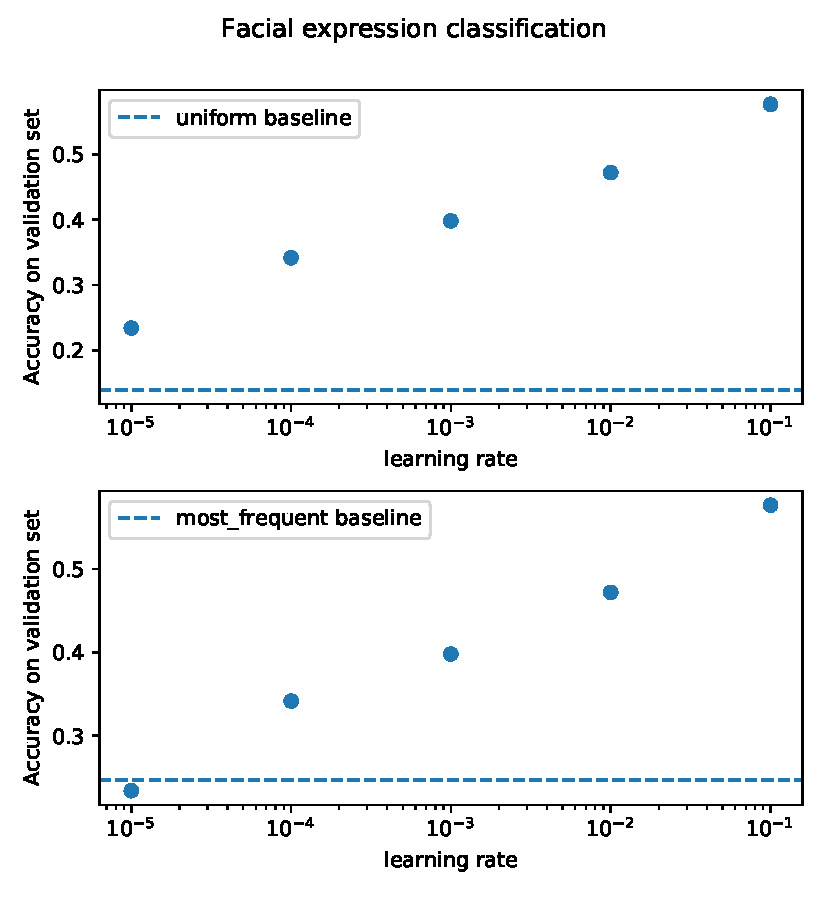
\includegraphics[width=\columnwidth]{figures/Resnet}
    \caption{Different learning rate versus Accuracy on validation set for Resnet-18 classifier}
    \label{fig:resnet_lr}
\end{figure}

At the same setting with SVM, the learning rates are compared with two dummy classifiers, a uniform baseline and a most-frequent baseline. According to figure \ref{fig:resnet_lr}, model with learning rate of 0.1 has the best performance on validation set. They all have better accuracy than two baselines except for learning rate of $10^{-5}$. We trained the model with 0.1 learning rate for 100 epoch and evaluated it on test set. We got accuracy of 0.574 which agreed with our expectation.

\iffalse
This section should cover the experiments carried out, including, for each experiment, the:
\begin{itemize}
    \item  Motivation -- what did you aim to learn from the experiment?
    \item  Baselines -- do you compare your method to appropriate baselines (e.g. the existing method that you built on your method)?
    \item  Description -- describe carefully how you carried out the experiment, mentioning and justifying the hyperparameter settings. As always, your aim is to give enough information so that someone else (e.g. another MLP group) could reproduce the experiment precisely.
    \item  Results -- present the results clearly and concisely. Usually a result is in comparison to a result from another approach (e.g. a baseline experiment, the previous experiment, results from the literature, \dots).  Please make sure that these comparisons are clearly presented.
    \item Interpretation and discussion -- what do your results indicate? how do they relate to the motivation for the experiment? are there further useful analyses or visualisations of the results that you can carry out?
\end{itemize}

Please note that negative results are not necessarily a bad thing -- learning is always good! But negative or positive, please try to analyse your results as well as you can.

There is no need to include code or specific details about the compute environment.

As before, your experimental sections should include graphs (for instance, figure~\ref{fig:resnet_lr}) and/or tables (for instance, table~\ref{tab:sample-table})\footnote{These examples were taken from the ICML template paper.}, using the \verb+figure+ and \verb+table+ environments, in which you use \verb+\includegraphics+ to include an image (pdf, png, or jpg formats).  Please export graphs as 
\href{https://en.wikipedia.org/wiki/Vector_graphics}{vector graphics}
rather than \href{https://en.wikipedia.org/wiki/Raster_graphics}{raster
files} as this will make sure all detail in the plot is visible.
Matplotlib supports saving high quality figures in a wide range of
common image formats using the
\href{http://matplotlib.org/api/pyplot_api.html\#matplotlib.pyplot.savefig}{\texttt{savefig}}
function. \textbf{You should use \texttt{savefig} rather than copying
the screen-resolution raster images outputted in the notebook.} An
example of using \texttt{savefig} to save a figure as a PDF file (which
can be included as graphics in a \LaTeX document is given in the coursework document.

If you need a figure or table to stretch across two columns use the \verb+figure*+ or \verb+table*+ environment instead of the \verb+figure+ or \verb+table+ environment.  Use the \verb+subfigure+ environment if you want to include multiple graphics in a single figure.



\begin{table}[tb]
\vskip 3mm
\begin{center}
\begin{small}
\begin{sc}
\begin{tabular}{lcccr}
\hline
\abovespace\belowspace
Data set & Naive & Flexible & Better? \\
\hline
\abovespace
Breast    & 95.9$\pm$ 0.2& 96.7$\pm$ 0.2& $\surd$ \\
Cleveland & 83.3$\pm$ 0.6& 80.0$\pm$ 0.6& $\times$\\
Glass2    & 61.9$\pm$ 1.4& 83.8$\pm$ 0.7& $\surd$ \\
Credit    & 74.8$\pm$ 0.5& 78.3$\pm$ 0.6&         \\
Horse     & 73.3$\pm$ 0.9& 69.7$\pm$ 1.0& $\times$\\
Meta      & 67.1$\pm$ 0.6& 76.5$\pm$ 0.5& $\surd$ \\
Pima      & 75.1$\pm$ 0.6& 73.9$\pm$ 0.5&         \\
\belowspace
Vehicle   & 44.9$\pm$ 0.6& 61.5$\pm$ 0.4& $\surd$ \\
\hline
\end{tabular}
\end{sc}
\end{small}
\caption{Classification accuracies for naive Bayes and flexible 
Bayes on various data sets.}
\label{tab:sample-table}
\end{center}
\vskip -3mm
\end{table}
\fi

\subsection{Robustness Test Results}
In this section, we will evaluate performance of SVM and ResNet-18 based on the robustness experiment results. When testing on the original test datasent, we achieve 48.97\% test accuracy using a SVM and 57.40\% using the ResNet18.

\begin{itemize}
    \item Add Gaussian pixel noise
    
    In Figure \ref{fig:gpn}, it can be seen that both models are tolerant to Gaussian pixel noises with relatively small standard deviation. It is also noticed that when increasing the standard deviation from 10 to 12, both models has a sudden drop in accuracy. 
    
    \begin{figure}[H]
    \centering
    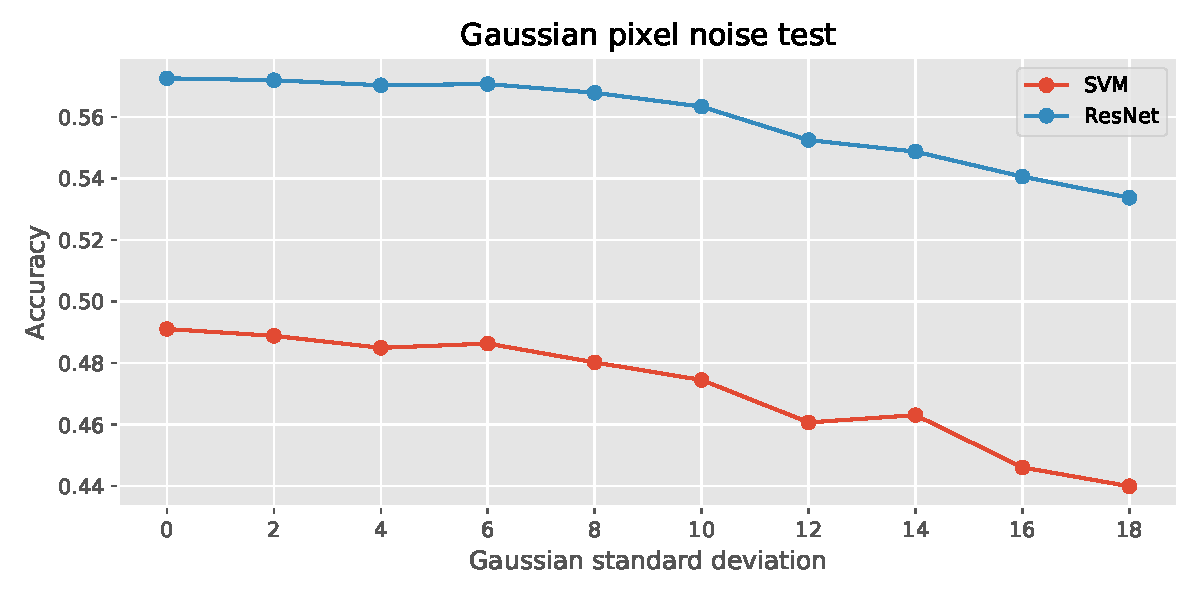
\includegraphics[width=\columnwidth]{figures/Gaussian_pixel_noise.pdf}
    \caption{Gaussian pixel noise}
    \label{fig:gpn}
    \end{figure}
    
    
    \item Gaussian blurring
    
    In Figure \ref{fig:gb}, we find that both classifiers cannot perform well on blurred image because their accuracy keeps shrinking to 0.30 along with successive Gaussian blurring operations.
    
    \begin{figure}[H]
    \centering
    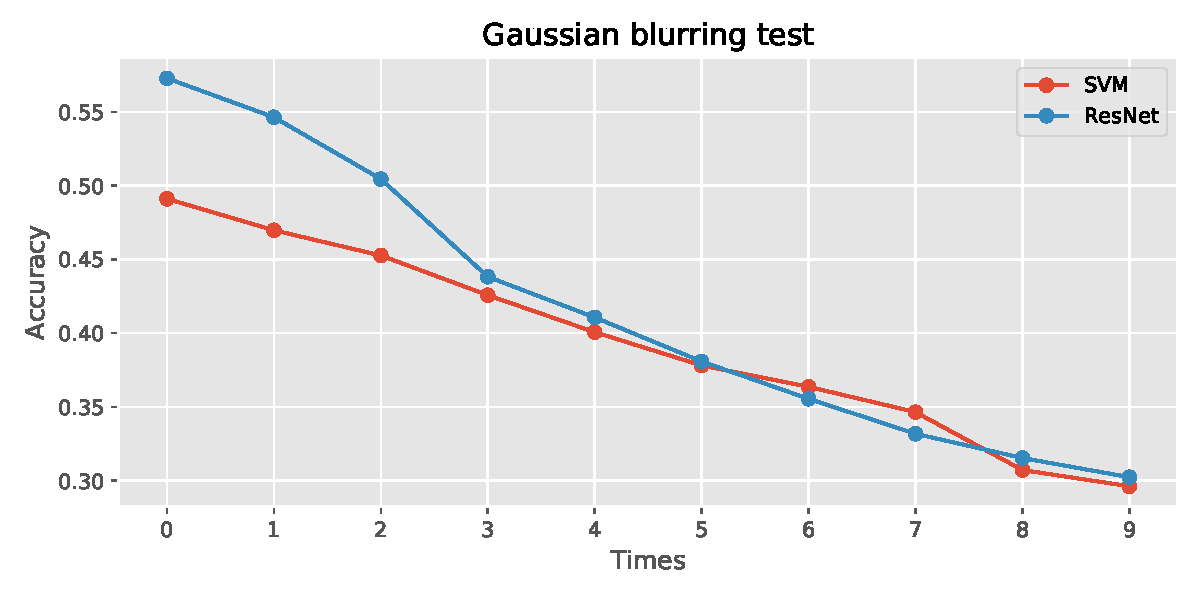
\includegraphics[width=\columnwidth]{figures/Gaussian_blurring.pdf}
    \caption{Gaussian blurring}
    \label{fig:gb}
    \end{figure}
    

    \item Image Contrast Increase
    
    In Figure \ref{fig:ici}, we can see that both classifiers are invariant to the increasing contrast perturbation in the given range. SVM performs slightly better in this case because there is a significant decrease of the ResNet accuracy when the contrast ratio is greater than 1.15, while the SVM maintains its accuracy at a high level.
    
    \begin{figure}[H]
    \centering
    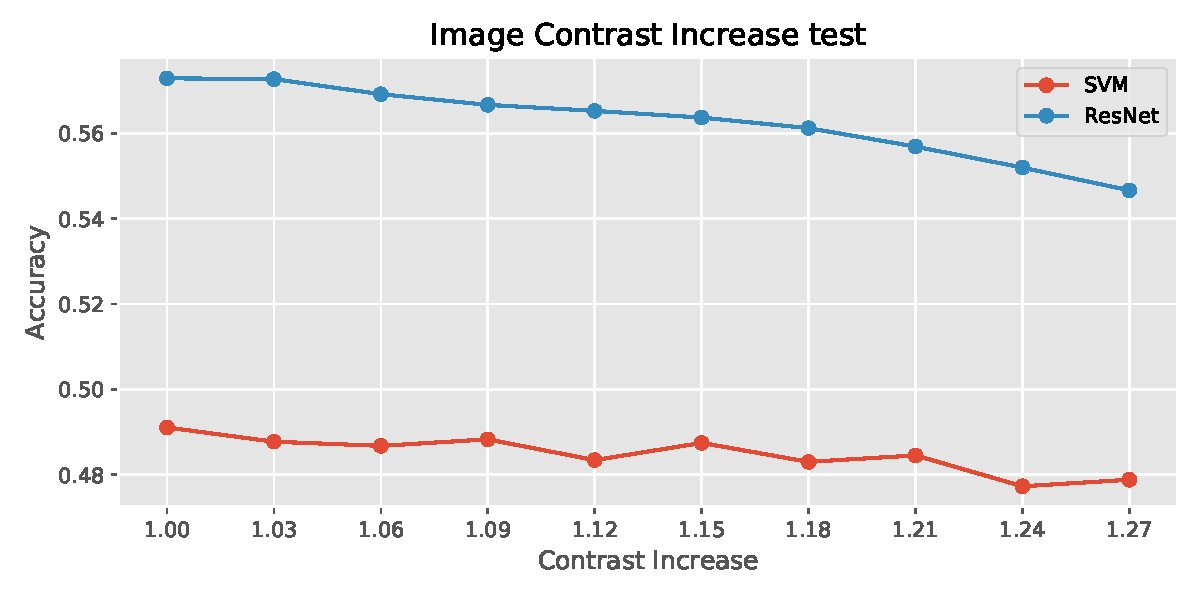
\includegraphics[width=\columnwidth]{figures/Image_Contrast_Increase.pdf}
    \caption{Image Contrast Increase}
    \label{fig:ici}
    \end{figure}
    
    
    \item Image Contrast Decrease
    
    In Figure \ref{fig:icd}, both models have a good performance before the image contrast decreases to 0.5. When the contrast ratio continues decreasing, there is a cliff-like drop in accuracy. The accuracy for SVM and ResNet is less than 0.2 on the highest perturbation level.
    
    \begin{figure}[H]
    \centering
    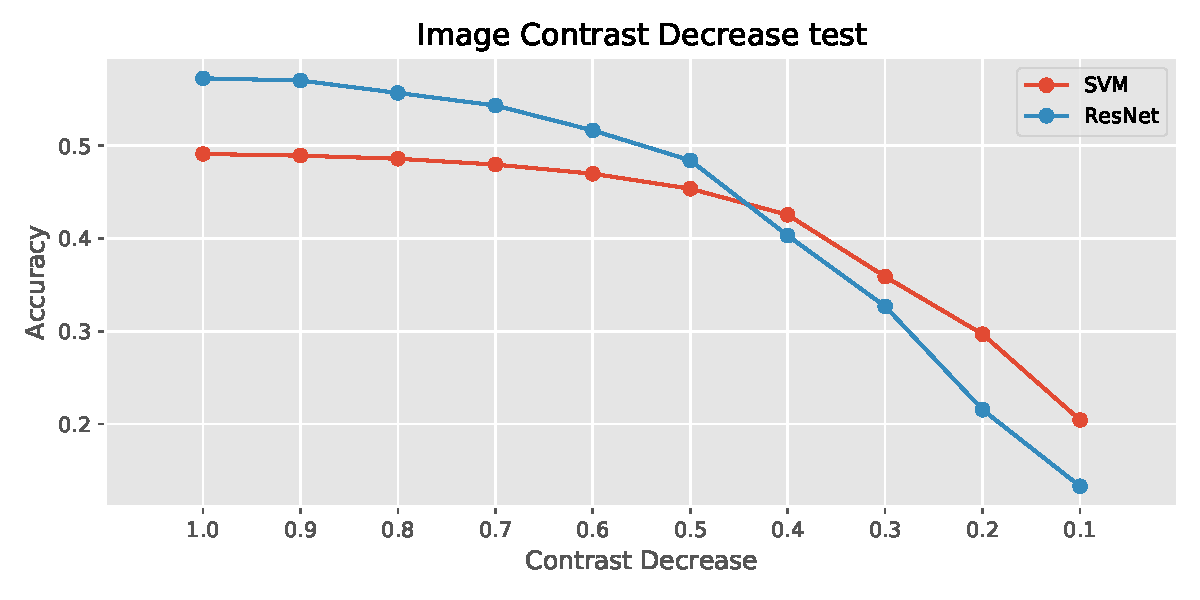
\includegraphics[width=\columnwidth]{figures/Image_Contrast_Decrease.pdf}
    \caption{Image Contrast Decrease}
    \label{fig:icd}
    \end{figure}
    

    \item Image Brightness Increase and Decrease
    
    In Figure \ref{fig:ibi} and Figure \ref{fig:ibd}, it can be seen that both models are immune to image brightness adjustments. SVM performs slightly better because its accuracy is stable while the accuracy of ResNet starts to decrease when the brightness is increased/decreased by 30.
    
    \begin{figure}[H]
    \centering
    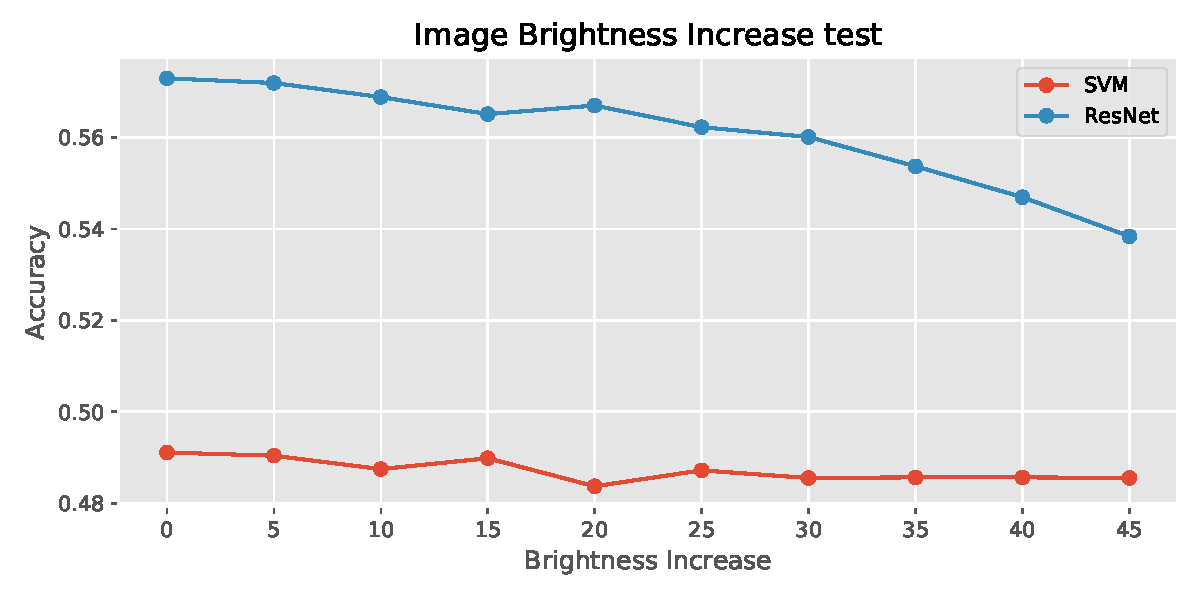
\includegraphics[width=\columnwidth]{figures/Image_Brightness_Increase.pdf}
    \caption{Image Brightness Increase}
    \label{fig:ibi}
    \end{figure}
    
    
    \begin{figure}[H]
    \centering
    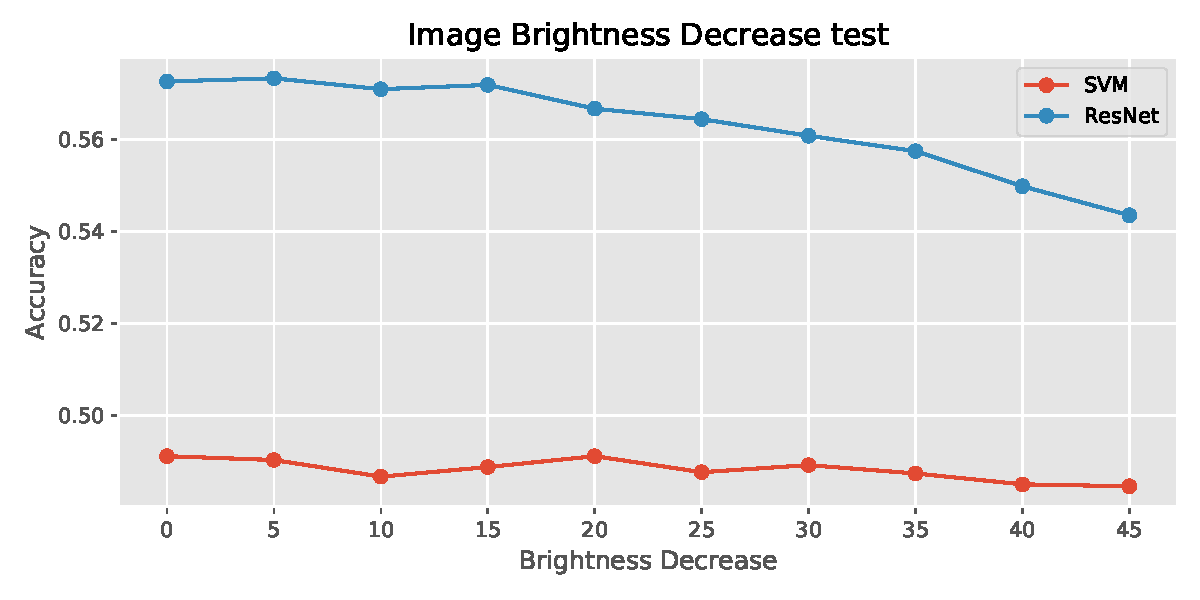
\includegraphics[width=\columnwidth]{figures/Image_Brightness_Decrease.pdf}
    \caption{Image Brightness Decrease}
    \label{fig:ibd}
    \end{figure}    

    \item Occlusion of the Image Increase
    
    From Figure \ref{fig:oi}, we can tell that both classifiers are vulnerable to occlusion attacks. The accuracy shrinks rapidly when the length of occlusion square edge increases.
    
    \begin{figure}[H]
    \centering
    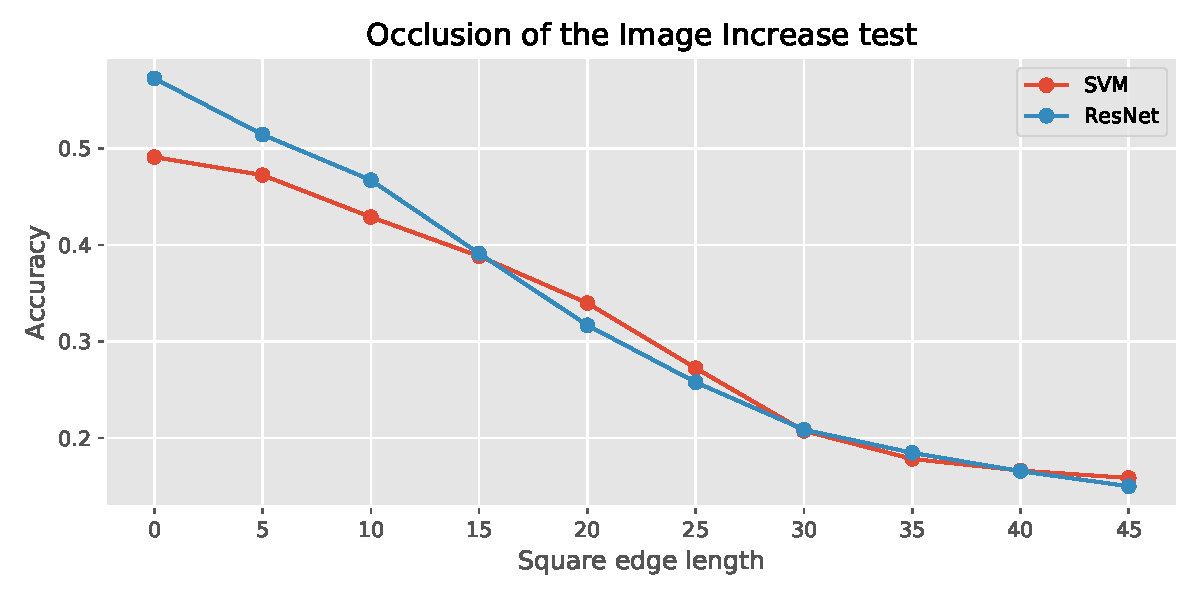
\includegraphics[width=\columnwidth]{figures/Occlusion_Increase.pdf}
    \caption{Occlusion of the Image Increase}
    \label{fig:oi}
    \end{figure}       

    \item Salt and Pepper Noise
    
    For salt and pepper noise test, the SVM classifier performs better because its accuracy is maintained at a relatively high level, while ResNet accuracy decreases from 0.57 to 0.44.
    
    \begin{figure}[H]
    \centering
    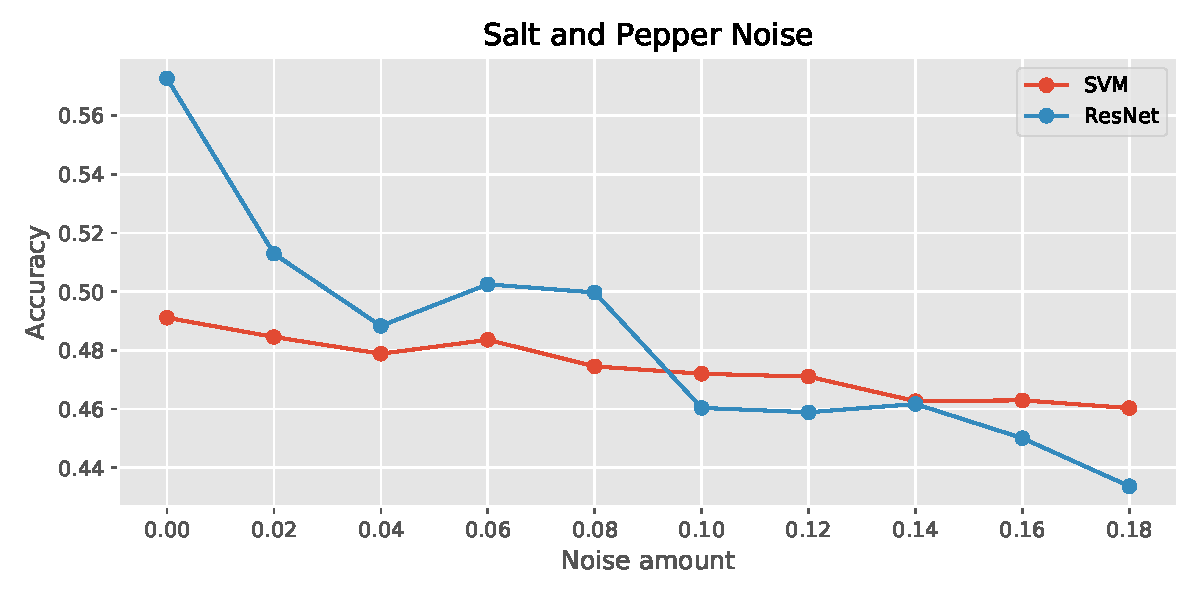
\includegraphics[width=\columnwidth]{figures/Salt_and_Pepper.pdf}
    \caption{Salt and Pepper Noise}
    \label{fig:sap}
    \end{figure}       
    
    
    \item Vertical comparison using the same model
    
    \begin{figure}[H]
    \centering
    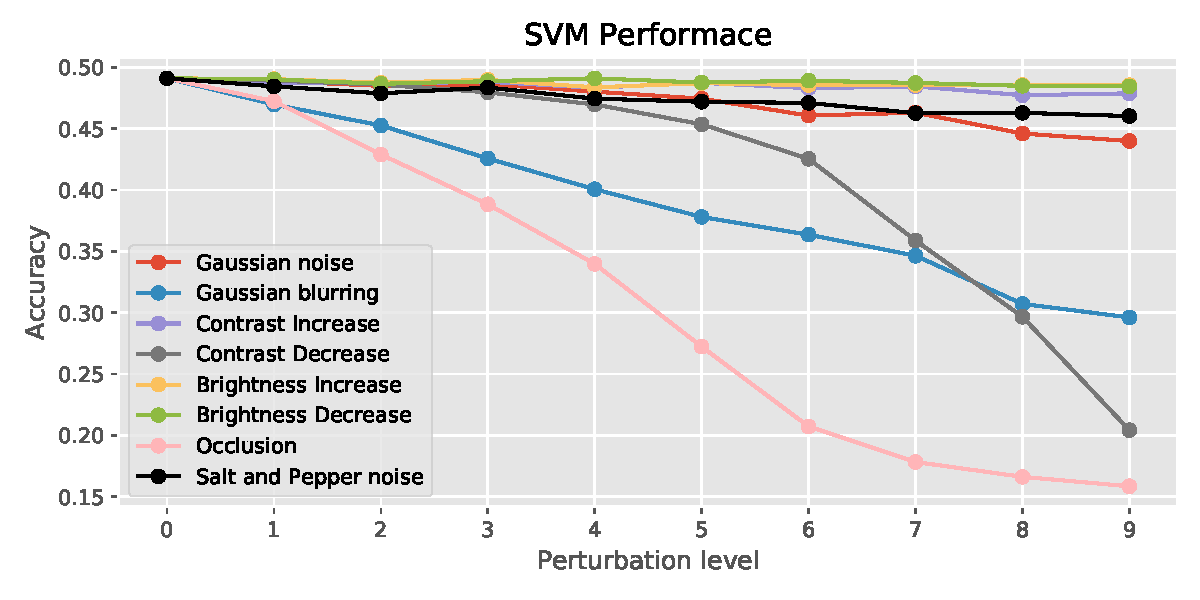
\includegraphics[width=\columnwidth]{figures/SVM_Performance.pdf}
    \caption{SVM Performance against perturbation}
    \label{fig:sp}
    \end{figure}        
    
    \begin{figure}[H]
    \centering
    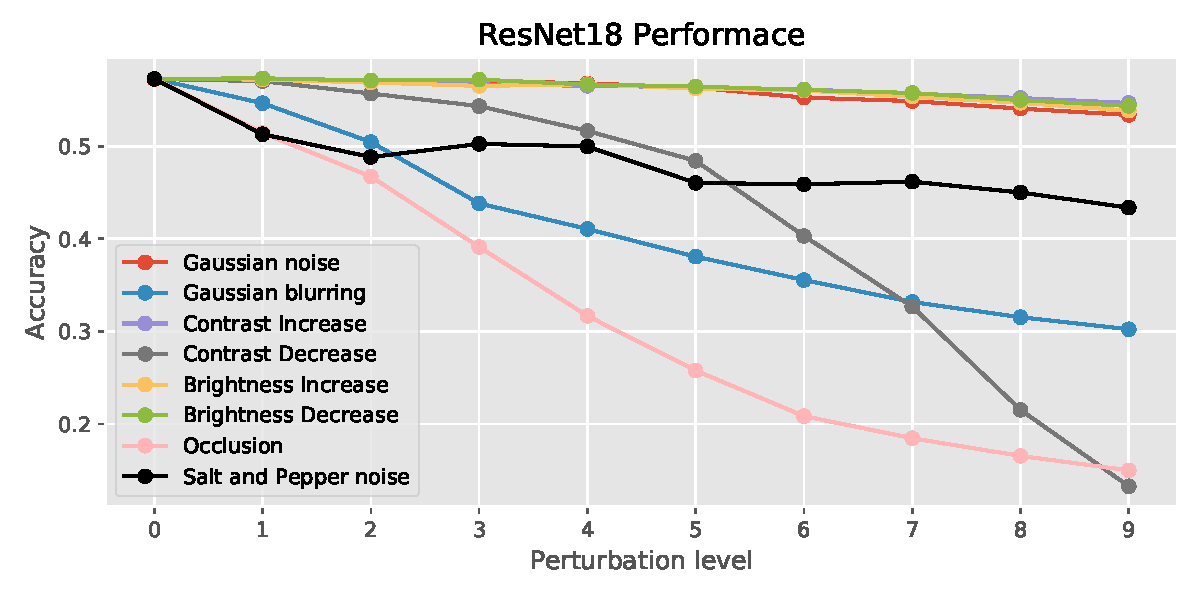
\includegraphics[width=\columnwidth]{figures/ResNet18_Performance.pdf}
    \caption{ResNet18 Performance against perturbation}
    \label{fig:rp}
    \end{figure}    

\end{itemize}


\section{Related work}
\label{sec:relwork}

In order to get a better understanding of how Resnet works we reviewed the article written by Kaiming He and his team which introduced deep residual learning for image recognition. This neural network won ILSVRC and COCO 2015 competitions and achieved 1st places in all five main tracks \citep{ImageNet}.

Comparing with other neural networks such as VGG and AlexNet, Resnet has the number of layers much more than them. As the number of layer increases, the neural network should be more capable of extracting complicated features. However many experiments show that neural networks with deeper layers has worse performance because of degradation problem. The accuracy are more likely saturated as the number of layer increased, while some regularisation method such as batch normalisation can't alleviate such problem.

In Resnet, Kaiming He uses some tricks to deal with accuracy degradation problem. He came up with a concept called residual learning. Given a few stacked non-linear layers with input $x$ and the learnt feature $H(x)$, we define a residual function $F(x)=H(x)-x$, and the learnt feature becomes $H(x)=F(x)+x$ \citep{ResnetReview}.

\begin{figure}[htp]
    \centering
    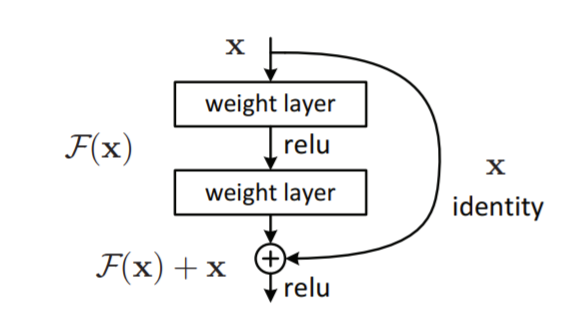
\includegraphics[width=\columnwidth]{figures/Residual learning.png}
    \caption{Residual learning building block}
    \label{fig:Residual learning}\citep{Resnet}
\end{figure}

Figure \ref{fig:Residual learning} shows the building block of residual learning. The inputs $x$ are directly connected with outputs of weight layer, which called short connection. The residual learning is easy than convolutional learning since it has smaller numbers to calculate. The basic residual units can be expressed in a general form:
\begin{align}
    y_l=h(x_l)+F(x_l+W_l)\\
    x_{l+1}=f(y_l)
\end{align}

While $x_l$ and $x_{l+1}$ the input and output of the $l^{th}$ residual unit, and $F$ is residual function representing what we learnt from stacked residual units. The function $h$ is identity mapping where $h(x_l)=x_l$. We could derive the equation for learnt feature from any shallower unit $l$ to deeper unit $L$:
\begin{align}
    X_L=X_l+\sum_{i=l}^{L-1}F(x_i,W_i)
\end{align}

Using chain rule, the gradient descent of loss function with respect to inputs is
\begin{align}
    \dfrac{\partial loss}{\partial x_l}=\dfrac{\partial loss}{\partial x_L}*\dfrac{\partial x_L}{\partial x_l} = \dfrac{\partial loss}{\partial x_L}*(1+\dfrac{\partial}{\partial x_l}\sum_{i=1}^{L-1}F(x_i,W_i))
\end{align}

The partial derivative term $\dfrac{\partial loss}{\partial x_L}$ represents the gradient of loss function of layer $L$. The number \textbf{1} in the bracket ensures that there is no gradient vanishing in shortcut connections and the other term in the bracket represents the residual gradients coming from layers with weights \citep{IdentityMappings}.

%This section should review published work which can help to give a better understanding of your work -- related approaches, other work on the same data, ideas for future work. The aim is to try to place what you have done in a wider context.

%The conclusions section should concisely summarise what you have learned from the experiments you carried out, and relate the final outcome of the project to the overall research questions and objectives. If there were potentially interesting future directions in your project that you could not explore due to lack of time and/or space, mention them briefly.

\section{Conclusions}
\label{sec:concl}
In this report, we have given the details about how the image features can be extrated using HOG and facial landmarks and then fed into SVM (and ResNet). We have explained the algorithms used for perturbing images. We have also compared the accuracy of SVM and ResNet based on original test data and further demonstrated how robust these two classifiers are according to their performance on the perturbed data.\\
As it is shown in Figure \ref{fig:sp} and Figure \ref{fig:rp}, we plot the performance of each model against different dataset with increasing level of perturbation. From these two figures, we can conclude that SVM and ResNet are robust against Gaussian noise, brightness changes and contrast increase. Besides, SVM is more invariant to salt and pepper noise than ResNet. Both models cannot overcome the challenges where there is a strong level of Gaussian blurring, contrast decrease or occlusion in the image.


\bibliography{example-refs}
\newpage
\thispagestyle{plain}

\onecolumn
\section{Appendix}
\subsection{Generating perturbations}
\begin{minted}
[
baselinestretch=1.2,
fontsize=\normalsize,
linenos,
breaklines
]
{python}
import numpy as np
from skimage.util import random_noise

# set seed
seed = 0
rng = np.random.RandomState(seed)

# fix pixel range and make sure all values are integer
def set_pixel_range(img):
    img[img>255] = 255
    img[img<0] = 0
    return img.astype(int)

# add Gaussian noise
def Gaussian_pixel_noise(std, img):
    noise_mask = rng.normal(0,std,size=(48,48)).astype(int)
    return set_pixel_range(img + noise_mask)

# convolution helper, used in Gaussian blur
def convole(image, kernel, average=False):

    image_row, image_col = image.shape
    kernel_row, kernel_col = kernel.shape
    
    #We will have the size of the output image same as that of the input image
    output = np.zeros(image.shape)
    
    #We will pad zeros around the boundaries around the image
    #This padding size maintains the image size
    pad_height = int((kernel_row - 1) / 2)
    pad_width = int((kernel_col - 1) / 2)

    #This is padded image (now are all zeros)
    padded_image = np.zeros((image_row + (2 * pad_height), image_col + (2 * pad_width)))
    #Fill the padded image with the values of the input image for corresponding pixels
    padded_image[pad_height:padded_image.shape[0] - pad_height, pad_width:padded_image.shape[1] - pad_width] = image
    
    #Here the convolution is performed. We have a window to slide over the padded image.
    for row in range(image_row):
         #From left to right
        for col in range(image_col):
            output[row, col] = np.sum(kernel * padded_image[row:row + kernel_row, col:col + kernel_col])
            if average:
                output[row, col] /= kernel.shape[0] * kernel.shape[1]

    return output


# Gaussian blur
def Gaussian_blurring(times,img):
    base_kernel = np.array([[1,2,1],[2,4,2],[1,2,1]])/16
    blur_image = img
    for i in range(times):
        blur_image = convole(blur_image, base_kernel)
        
    return set_pixel_range(blur_image)


# change image contrast 
def Image_Contrast(contrast, img):
    return set_pixel_range(img * contrast)

# change image brightness
def Image_Brightness(brightness, img):
    return set_pixel_range(img + brightness)

# add occlusion
def Occlusion(length, img):
    x = rng.randint(low=0, high=len(img)-length)
    y = rng.randint(low=0, high=len(img)-length)
    output = img.copy()
    
    output[x:x+length, y:y+length] = 0
    
    return output

# add salt and pepper noise
def Salt_and_Pepper_Noise(amount, img):
    noise = 255*random_noise(img, seed=seed,mode='s&p',amount =  amount)
    return set_pixel_range(noise)
)
\end{minted}


\subsection{training Resnet-18}

\begin{minted}
[
baselinestretch=1.2,
fontsize=\normalsize,
linenos,
breaklines
]
{python}
# set features in fully connected layer
fc_features = model.fc.in_features
model.fc = nn.Linear(fc_features, len(IMAGE_CATEGORIES))
# set input channel for conv1
model.conv1= nn.Conv2d(1, 64, kernel_size=(7,7), stride=(2,2), padding=(3,3),bias=False)
# setup the loss fxn
criterion = nn.CrossEntropyLoss()
device = torch.device('cuda:0' if torch.cuda.is_available() else 'cpu')
model = model.to(device)
optimizer = torch.optim.SGD(model.parameters(), lr=0.1)
# make_dataloader function produces DataLoader files for Resnet
train_loader = make_dataloader(train_images, train_labels_encode, 100, True)
valid_loader = make_dataloader(validation_images, validation_labels_encode, 100, False)
test_loader = make_dataloader(test_images, test_labels_encode, 100, False)
# train the model for 100 epoch
train_model(model, criterion, optimizer, train_loader, valid_loader, epochs=100)

# plot accuracy on validation set with different learning rates
from sklearn.dummy import DummyClassifier

baselines = ['uniform', 'most_frequent']
fig, ax = plt.subplots(len(baselines), 1, figsize=(5.5,6))

for ii, baseline in enumerate(baselines):
    category = []
    plt.sca(ax[ii])
    dummy_classifier = DummyClassifier(strategy=baseline).fit(test_images, test_labels_encode)
    pred_proba = dummy_classifier.predict_proba(test_images)
    for i in range(pred_proba.shape[0]):
      category.append(np.random.choice(np.arange(pred_proba[i].size),p=pred_proba[i]))
    equals = (category == test_labels_encode)
    acc = equals.sum()/len(test_labels_encode)

    plt.axhline(acc, label='{} baseline'.format(baseline), linestyle='--')
    plt.scatter(lr, accuracy)
    plt.xscale('log')
    plt.xlabel('learning rate')
    plt.ylabel('Accuracy on validation set')
    plt.legend()
plt.savefig("Resnet.pdf")
plt.suptitle('Facial expression classification')
plt.tight_layout()
plt.subplots_adjust(top=0.9)
plt.savefig("Resnet.pdf")
plt.show()

\end{minted}

\subsection{training SVM}

\begin{minted}
[
baselinestretch=1.2,
fontsize=\normalsize,
linenos,
breaklines
]
{python}
# read one image to see its size
img = cv2.imread(train_image_paths[0])
#hyperparameters
shape_x = img.shape[0]
shape_y = img.shape[1]
ORIENTATIONS = 8
PIXES_PER_CELL = (16, 16)
CELLS_PER_BLOCK = (3, 3)

# extrac HOG features from images
def hog_feagures_extraction(input_images):
  hog_features = []
  train_hog_images = []
  for i in range(len(input_images)):
    img = input_images[i].reshape((shape_x, shape_y))
    features, hog_image = hog(
        img,
        orientations = ORIENTATIONS,
        pixels_per_cell = PIXES_PER_CELL,
        cells_per_block = CELLS_PER_BLOCK,
        visualize = True)
    hog_features.append(features)
    hog_images.append(hog_image)
    return hog_features, hog_images
train_hog_features, _ = hog_feagures_extraction(train_images)
validation_hog_features, _ = hog_feagures_extraction(validation_images)
test_hog_features, _ = hog_feagures_extraction(test_images)

# concatenate landmarks with image
X = np.hstack((train_hog_features,train_landmarks))
np.shape(X)
X_test = np.hstack((test_hog_features,test_landmarks))
np.shape(X_test)

model = svm.SVC(decision_function_shape='ovo', random_state=42, max_iter=10000, kernel='rbf',gamma='auto')

start_time = time()
X,y = shuffle(X,train_labels)
model.fit(X,y)
training_time = time() - start_time
print("Training time : ", training_time)

# Predict
y_pred = model.predict(X_test)
accuracy_landmarks = accuracy_score(y_pred, test_labels)
print("Accuracy : ", accuracy_landmarks)

# plot accuracy on validation set with different pixels per cell
pixel = ['12x12', '16x12', '16x16', '24x16', '24x24']
baselines = ['uniform', 'most_frequent']
fig, ax = plt.subplots(len(baselines), 1, figsize=(5.5,6))

for ii, baseline in enumerate(baselines):
    category = []
    plt.sca(ax[ii])
    dummy_classifier = DummyClassifier(strategy=baseline).fit(test_images, test_labels_encode)
    pred_proba = dummy_classifier.predict_proba(test_images)
    for i in range(pred_proba.shape[0]):
      category.append(np.random.choice(np.arange(pred_proba[i].size),p=pred_proba[i]))
    equals = (category == test_labels_encode)
    acc = equals.sum()/len(test_labels_encode)
    plt.axhline(acc, label='{} baseline'.format(baseline), linestyle='--')
    plt.plot(pixel, accuracy, 'o')
    plt.xlabel('PIXES_PER_CELL')
    plt.ylabel('Accuracy on validation set')
    plt.legend()

plt.suptitle('Facial expression classification')
plt.tight_layout()
plt.subplots_adjust(top=0.9)
plt.savefig("SVM.pdf")
plt.show()
\end{minted}

\end{document} 


